\documentclass{beamer}

\usepackage[utf8]{inputenc}
\usepackage[T1]{fontenc}

\usepackage{graphicx}
\usepackage[french]{babel}
\usepackage{comment}

\usepackage{booktabs}
% Quelle fontes de caractères
%\usepackage{lmodern}
\usepackage{inconsolata}

% pour insérer directement des fig
\usepackage{figlatex}

% où se trouvent les images
\graphicspath{{images/}{pdfs/}{figs/}{svgs/}{odgs/}}

% pour ne pas mettre l'extension des images
\DeclareGraphicsExtensions{.fig,.pdf,.png,.jpg}

% beamer theme
\mode<presentation>
% If you want headline with section list
%\usetheme[infolines]{tptnew}
% If you want to add "Université Paris Saclay" logos
%\usetheme[logosaclay]{tptnew}
\usetheme{tptnew}


%%------------------------------------------------------------------------------
\begin{comment}
%% Faire apparaitre le plan à chaque section
\AtBeginSection[]
{
    \begin{frame}<beamer>
        \frametitle{Plan}
        \tableofcontents[currentsection]
        \end{frame}
}
\AtBeginSubsection[]
{
    \begin{frame}<beamer>
        \frametitle{Plan}
        \tableofcontents[currentsubsection]
        \end{frame}
}
\end{comment}
%------------------------------------------------------------------------------


%------------------------------------------------------------------------------
\title{Find and fix security flaws using formal methods}
\subtitle{V4}

\author{A. Anselmo, S. A. Chiaberto, G. Roggero}
\institute{EURECOM}
\extralogo{
\includegraphics[width=2cm]{logo-EURECOM}}
\date{17-01-2019}
%------------------------------------------------------------------------------
\begin{document}

\maketitle

%------------------------------------------------------------------------------
\section[1e] { 1e Section }
%------------------------------------------------------------------------------
\subsection[1su] { Sous section 1}
%------------------------------------------------------------------------------
\begin{frame}
\frametitle{First Frame}

\begin{itemize}
\item bla bla bla
  \begin{itemize}
    \item bla bla bla
    \item bla bla bla
  \end{itemize}
\item bla bla bla
\end{itemize}

\end{frame}
%------------------------------------------------------------------------------
\begin{frame}
\frametitle{an other Frame}
\framesubtitle{sub title}

\begin{itemize}
\item bla bla bla
  \begin{itemize}
    \item bla bla bla
    \item bla bla bla
  \end{itemize}
\item bla bla bla
\end{itemize}

\end{frame}
%------------------------------------------------------------------------------
\begin{frame}
\frametitle{an other Frame}

\begin{center}
  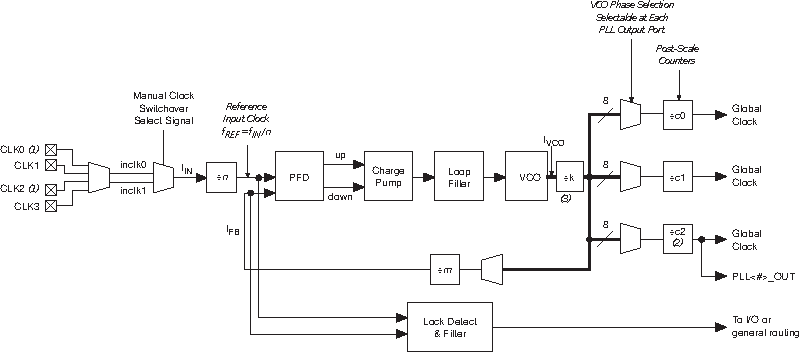
\includegraphics[width=\textwidth]{cycii_PLL}
\end{center}

\end{frame}
%------------------------------------------------------------------------------
\begin{frame}
\frametitle{an other Frame from an \texttt{odg}}

\begin{center}
   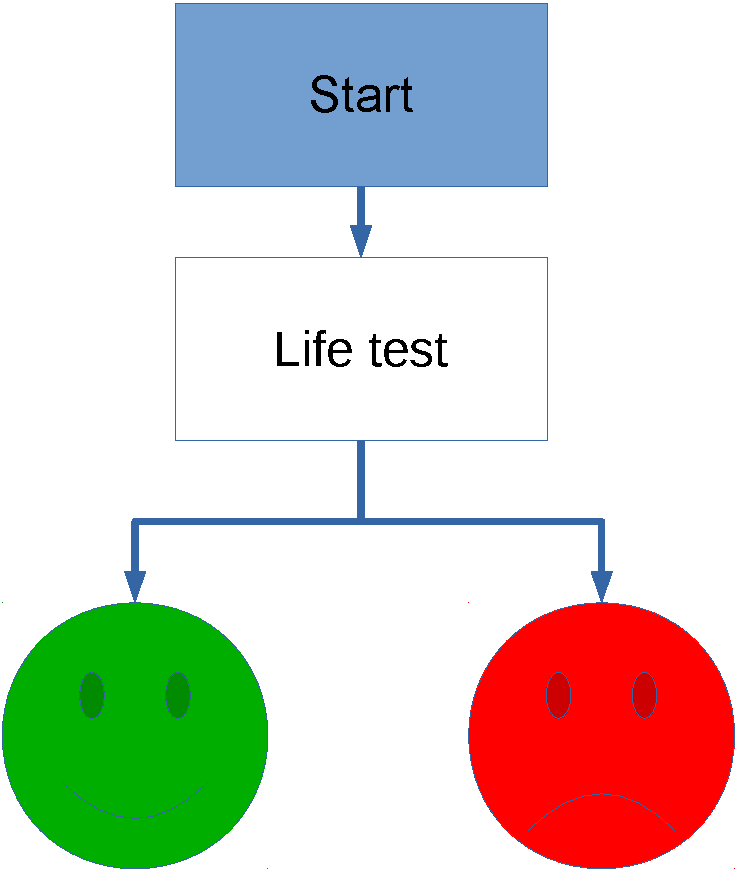
\includegraphics[height=.8\textheight,width=\textwidth,keepaspectratio]{diag}
\end{center}

\end{frame}
%------------------------------------------------------------------------------
\begin{frame}
   \frametitle{an SVG illustration}

\begin{center}
   
\includegraphics[height=.8\textheight]{drawing}
\end{center}

\end{frame}
%------------------------------------------------------------------------------
\subsection { Sous section 2}
%------------------------------------------------------------------------------
\begin{frame}
\frametitle{an other Frame}

\begin{center}
  \includegraphics[width=\textwidth]{fpga-dff}
\end{center}

\end{frame}
%------------------------------------------------------------------------------
\section[2e] { 2e Section }
%------------------------------------------------------------------------------
\begin{frame}
\frametitle{First Frame}

\begin{itemize}
\item bla bla bla
  \begin{itemize}
    \item bla bla bla
    \item bla bla bla
  \end{itemize}
\item bla bla bla
\end{itemize}

\end{frame}
%------------------------------------------------------------------------------
\subsection { Sous section 1}
%------------------------------------------------------------------------------
\begin{frame}
\frametitle{an other Frame}

\begin{itemize}
\item bla bla bla
  \begin{itemize}
    \item bla bla bla
    \item bla bla bla
  \end{itemize}
\item bla bla bla
\end{itemize}

\end{frame}
%------------------------------------------------------------------------------
\subsection { Sous section 2}
%------------------------------------------------------------------------------
\begin{frame}
\frametitle{an other Frame}

\begin{itemize}
\item bla bla bla
  \begin{itemize}
    \item bla bla bla
    \item bla bla bla
  \end{itemize}
\item bla bla bla
\end{itemize}

\end{frame}
%------------------------------------------------------------------------------
\section[3e] { 3e Section }
%------------------------------------------------------------------------------
\begin{frame}
\frametitle{Block Frame}

\begin{block}{This is a block}
\begin{itemize}
\item bla bla bla
  \begin{itemize}
    \item bla bla bla
    \item bla bla bla
  \end{itemize}
\item bla bla bla
\end{itemize}
\end{block}

\end{frame}
%------------------------------------------------------------------------------
\begin{frame}
\frametitle{AlertBlock Frame}

\begin{alertblock}{This is a block}
\begin{itemize}
\item bla bla bla
  \begin{itemize}
    \item bla bla bla
    \item bla bla bla
  \end{itemize}
\item bla bla bla
\end{itemize}
\end{alertblock}

\end{frame}

\end{document}
